\section{Supervised Machine Learning}\label{sec:ch2:supervised}
While this subject is general and covered in many places, we take inspiration
from \cite{murphy_machine_2012} (chapters 1, 2, 7, 8) and
\cite{goodfellow_deep_2016} (chapter 5-10).
Consider a sample space over inputs and targets $\mathcal{X} \times \mathcal{Y}$
and a data generating distribution $p_{data}$. Given a dataset of input-target
pairs $\mathcal{D} = \{(x^{(n)}, y^{(n)})\}_{n=1}^N$ we would like to make
predictions about $p_{data}(y|x)$ that generalize well to unseen data. A common
way to do this is to build a parametric model to directly estimate this
conditional probability.  For example, regression asserts the data are
distributed according to a function of the inputs plus a noise term $\epsilon$:
\begin{equation}
  y = f(x, \theta) + \epsilon
\end{equation}
This noise is often modelled as a zero-mean Gaussian random variable, $\epsilon
\sim \mathcal{N}(0, \sigma^2I)$, which means we can write:
\begin{equation}\label{eq:ch2:regression}
  p_{model}(y|x, \theta, \sigma^2) = \mathcal{N}(y;\ f(x, \theta), \sigma^2I)
\end{equation}
where $(\theta, \sigma^2)$ are the parameters of the model.

We can find point estimates of the parameters by maximizing the likelihood of
$p_{model}(y|x, \theta)$ (or equivalently, minimizing $KL(p_{model}||p_{data})$, the KL-divergence between
$p_{model}$ and $p_{data}$). As the data are all assumed to be
i.i.d., we can multiply individual likelihoods, and solve for $\theta$:
\begin{align}
  \theta_{MLE} &= \argmax_{\theta} p_{model}(y|x, \theta) \\
              &= \argmax_{\theta} \prod_{n=1}^{N} p_{model}(y^{(n)}|x^{(n)}, \theta) \\
              &= \argmax_{\theta} \sum_{n=1}^N \log p_{model}(y^{(n)}|x^{(n)}, \theta)
\end{align}
Using the Gaussian regression model from above, this becomes:
\begin{align}
  \theta_{MLE} &= \argmax_{\theta} \sum_{n=1}^N \log p_{model}(y^{(n)}|x^{(n)}, \theta) \\
              &= \argmax_{\theta} \left(-N\log \sigma - \frac{N}{2}\log (2\pi) - \sum_{n=1}^{N}
                  \frac{\left(y^{(n)} - f(x^{(n)}, \theta)\right)^2}{2\sigma^2}\right) \\
                  &= \argmin_{\theta}\frac{1}{N}\sum_{n=1}^{N} \frac{\left(y^{(n)} - f(x^{(n)}, \theta)\right)^2}{2} \label{eq:ch2:mle_reg}
\end{align}
which gives us the well-known result that we would like to find parameters that
minimize the mean squared error (MSE) between targets $y$ and predictions
$\hat{y} = f(x, \theta)$.

For binary classification $y \in \{0, 1\}$ and instead of the model in
\eqref{eq:ch2:regression}, we have:
\begin{equation} \label{eq:ch2:logistic}
  p_{model}(y|x, \theta) = \F{Ber}(y;\ \sigma(f(x, \theta)))
\end{equation}
where $\sigma(x)$ is the sigmoid function and $\F{Ber}$ is the Bernoulli
distribution. Note that we have used $\sigma$ to refer to noise standard
deviation thus far but now use $\sigma(x)$ to refer to the sigmoid and softmax
functions, a confusing but common practice. $\sigma(x)$ and
$\F{Ber}(y; p)$ are defined as:
\begin{align}
  \sigma(z) &= \frac{1}{1+e^{-z}} \label{eq:ch2:sigmoid} \\
  \F{Ber}(y; p) &= p^{\indic(y=1)}(1-p)^{\indic(y=0)}
\end{align}
where $\indic(x)$ is the indicator function. The sigmoid function is useful here
as it can convert a real output $f(x, \theta)$ into a probability estimate.
In particular, large positive values get mapped to 1, large negative values to
0, and values near 0 get mapped to 0.5 \cite[Chapter~6]{goodfellow_deep_2016}.

This expands naturally to multi-class classification by making $y$ a 1-hot
vector in $\{0, 1\}^C$. We must also
swap the Bernoulli distribution for the Multinoulli or Categorical distribution,
and the sigmoid function for a softmax. The softmax function for vector $\bm{z}$
is defined as:
\begin{equation}
  \sigma_i(\bm{z}) = \frac{e^{z_i}}{\sum_{k=1}^C e^{z_k}} \\
\end{equation}
which has the nice properties that $0 \leq \sigma_i \leq 1$ and $\sum_i \sigma_i = 1$. The categorical
distribution uses the softmax output:
\begin{equation}
  \F{Cat}(y; \bm{\sigma}) = \prod_{c=1}^C \sigma_c^{\indic(y_c = 1)}
\end{equation}
If we let $\hat{y}_c = \sigma_c(f(x, \theta))$, this makes \eqref{eq:ch2:logistic}:
\begin{align}\label{eq:ch2:classification}
  p_{model}(y|x, \theta) &= \F{Cat}(y;\ \sigma(f(x, \theta))) \\
                         &= \prod_{c=1}^C \prod_{n=1}^N \left(\hat{y}_c^{(n)}\right)^{\indic(y^{(n)}_c = 1)}
\end{align}
As $y^{(n)}_c$ is either 0 or
1, we remove the indicator function. Maximizing this likelihood to
find the ML estimate for $\theta$:
\begin{align}
  \theta_{MLE} &= \argmax_\theta \prod_{c=1}^C \prod_{n=1}^N \left(\hat{y}_c^{(n)}\right)^{y^{(n)}_c} \\
               &= \argmax_\theta \frac{1}{N}\sum_{n=1}^N \sum_{c=1}^C y^{(n)}_c\log \hat{y}_c^{(n)} \label{eq:ch2:mle_class}
\end{align}
which we recognize as the cross-entropy between $y$ and $\hat{y}$.

\subsection{Priors on Parameters and Regularization}
  Maximum likelihood estimates for parameters, while straightforward, can often
  lead to overfitting. A common practice is to regularize learnt parameters
  $\theta$ by putting a prior over them. If we do not have any prior information
  about what we expect them to be, it may still be useful to put an
  uninformative prior over them. For example, if our parameters are in the
  reals, a commonly used uninformative prior is a Gaussian.

  Let us extend the regression example from above by saying we would like the
  prior on the parameters $\theta$ to be a Gaussian, i.e.
  $p(\theta) = \mathcal{N}(0, \tau^2I_D)$. The corresponding maximum a posteriori
  (MAP) estimate is then obtained by finding:
  \begin{align}\label{eq:ch2:map}
    \theta_{MAP} &= \argmax_\theta\ p(\theta | \mathcal{D}, \sigma^2) \\
                 &= \argmax_\theta\ \frac{p(y| x, \theta, \sigma^2) p(\theta)}{p(y|x)} \\
                 &= \argmax_\theta\ \log p(y|x, \theta, \sigma^2) + \log p(\theta) \\
                 &= \argmin_{\theta}\ \frac{1}{N}\sum_{n=1}^{N} \frac{\left(y^{(n)} - f(x^{(n)}, \theta)\right)^2}{2} +
      \frac{\lambda}{2} ||\theta||_2^2
  \end{align}
  where $\lambda = \sigma^2/\tau^2$ is the ratio of the observation noise to the
  strength of the prior \cite[Chapter~7]{murphy_machine_2012}. This is
  equivalent to minimizing the MSE with an $\ell_2$ penalty on the parameters,
  also known as ridge regression or penalized least squares.
  $\lambda$ is often called \emph{weight decay} in the neural network
  literature, which we will also use in this thesis.

\subsection{Loss Functions and Minimizing the Objective}
  It may be useful to rewrite \eqref{eq:ch2:map} as an objective function on the
  parameters $J(\theta)$:
  \begin{align}
    J(\theta) &=\frac{1}{N}\sum_{n=1}^{N} \frac{\left(y^{(n)} - f(x^{(n)}, \theta)\right)^2}{2} +
                  \frac{\lambda}{2} ||\theta||_2^2 \label{eq:ch2:regression_ob} \\
              &= L_{data}(y, f(x, \theta)) + L_{reg}(\theta) \label{eq:ch2:objective}
  \end{align}
  where $L_{data}$ is the data loss such as MSE or cross-entropy and
  $L_{reg}$ is the regularization, such as $\ell_2$ or $\ell_1$ penalized loss.
  Now $\theta_{MAP} = \argmin_\theta J(\theta)$.

  Finding the global minimum of the objective
  function is task-dependent and is often not straightforward. One commonly used
  technique is called \emph{gradient descent} (GD). This is not difficult to do as
  it only involves calculating the gradient at a given point and taking a small
  step in the direction of steepest descent. The update equation for GD is:
  \begin{equation}\label{eq:ch2:gd}
    \theta_{t+1} = \theta_t - \eta \dydx{J}{\theta}
  \end{equation}
  Unsurprisingly, such a simple technique has limitations. In particular, it
  is sensitive to the choice of step size and
  has a slow convergence rate when the condition number (ratio of largest to
  smallest eigenvalues) of the Hessian around the optimal point is large
  \cite{boyd_convex_2004}. An example of this is shown in
  \autoref{fig:ch2:gd_bounce}. In this figure, the step size is chosen with
  exact line search, i.e.
  \begin{equation}\label{eq:ch2:search}
    \eta = \argmin_s f(x + s \dydx{f}{x})
  \end{equation}

  To truly overcome this problem, we must know the curvature
  of the objective function $\frac{\partial^2 J}{\partial \theta^2}$. An example
  optimization technique that uses the second-order information is Newton's
  method \cite[Chapter~9]{boyd_convex_2004}. Such techniques sadly do not scale
  with size, as computing the Hessian is proportional to the number of
  parameters squared, and many neural networks have hundreds of thousands, if
  not millions of parameters. In this thesis, we only consider
  \emph{first-order} optimization algorithms.

  \begin{figure}[t]
  \centering
  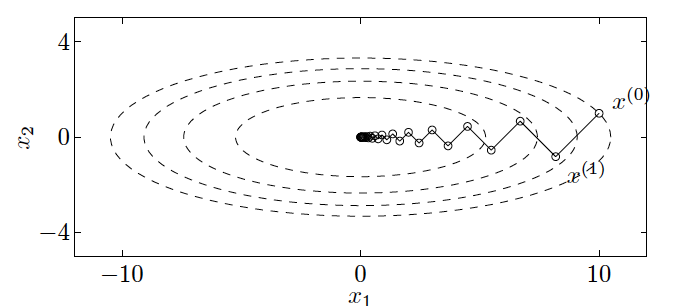
\includegraphics[width=0.8\textwidth]{\imgpath/sgd_bounce.png}
  \mycaption{Trajectory of gradient descent in an ellipsoidal parabola}{Some contour lines of
  the function $f(x)=1/2\left(x_1^2 + 10x_2^2 \right)$ and the trajectory of GD
  optimization using exact line search.
  This space has condition number 10, and shows the slow convergence of GD in
  spaces with largely different eigenvalues.
  Image is taken from \cite{boyd_convex_2004} Figure 9.2.}
  \label{fig:ch2:gd_bounce}
\end{figure}

\subsection{Stochastic Gradient Descent}
Aside from the problems associated with the curvature of the function $J(\theta)$,
another common issue faced with the gradient descent of \eqref{eq:ch2:gd} is the
cost of computing $\dydx{J}{\theta}$. In particular, the first term:
\begin{align}\label{eq:ch2:ldata}
  L_{data}(y, f(x, \theta)) &= \mathbb{E}_{x,y \sim p_{data}}\left[ L_{data}(y, f(x, \theta))\right] \\
                            &= \frac{1}{N}\sum_{n=1}^N L_{data}\left(y^{(n)}, f(x^{(n)}, \theta)\right)
\end{align}
involves evaluating the entire dataset at the current values of $\theta$. As the
training set size grows into the thousands or millions of examples, this
approach becomes prohibitively slow.

\eqref{eq:ch2:ldata} writes the data loss as an expectation, hinting at the fact that
we can remedy this problem by using fewer samples $N_b < N$ to evaluate $L_{data}$.
This variation is called Stochastic Gradient Descent (SGD).

Choosing the batch size is a hyperparameter choice that we must think carefully
about. Setting the value very low, e.g. $N_b = 1$ can be advantageous as the
noisy estimates for the gradient have a regularizing effect on the network
\cite{wilson_general_2003}. Increasing the batch size to larger values allows
you to easily parallelize computation as well as increasing your accuracy for
the gradient, allowing you to take larger step sizes \cite{smith_dont_2017}.
A good initial starting point is to set the batch size to 128 samples and
increase/decrease from there \cite{goodfellow_deep_2016}.

\subsection{Gradient Descent and Learning Rate}
The step size parameter, $\eta$ in \eqref{eq:ch2:gd} is commonly referred to as
the learning rate. Choosing the right value for the learning rate is key.
Unfortunately, the line search algorithm in \eqref{eq:ch2:search} would be too
expensive to compute for neural networks (as it would involve evaluating the
function several times at different values), each of which takes about as long
as calculating the gradients themselves. Additionally, as the gradients are
typically estimated over a mini-batch and are hence noisy there may be
little added benefit in optimizing the step sizes in the estimated direction.

\autoref{fig:ch2:sgd_lr} illustrates the effect the learning rate can have over
a contrived convex example. Optimizing over more complex loss surfaces only
exacerbates the problem. Sadly, choosing the initial learning rate is
`more of an art than a science' \cite{goodfellow_deep_2016}, but
\cite{bottou_stochastic_2012-1, montavon_neural_2012} have some tips on what to
how to set it. We have found in our work that searching for a large learning
rate that causes the network to diverge and reducing it from there can be a good
search strategy. This agrees with Section 1.5 of \cite{lecun_efficient_2012}
which states that for regions of the loss space which are roughly quadratic,
$\eta_{max} = 2\eta_{opt}$ and any learning rate above $2\eta_{opt}$ causes
divergence.

On top of the initial learning rate, the convergence of SGD methods require
\cite{bottou_stochastic_2012-1}:
\begin{align}
  \sum_{t=1}^{\infty} \eta_t &\rightarrow \infty \\
  \sum_{t=1}^{\infty} \eta_t^2 &< \infty
\end{align}
Choosing how to do this also contains a good amount of artistry,
and there is no one scheme that works best. A commonly used greedy method is to
keep the learning rate constant until the training loss stabilizes and then to
enter the next phase of training by setting $\eta_{k+1} = \gamma \eta_{k}$ where
$\gamma$ is a decay factor. Setting $\gamma$ and the thresholds for triggering
a step however must be chosen by monitoring the training loss curve and trial
and error \cite{bottou_stochastic_2012-1}.

\begin{figure}[t]
  \centering
  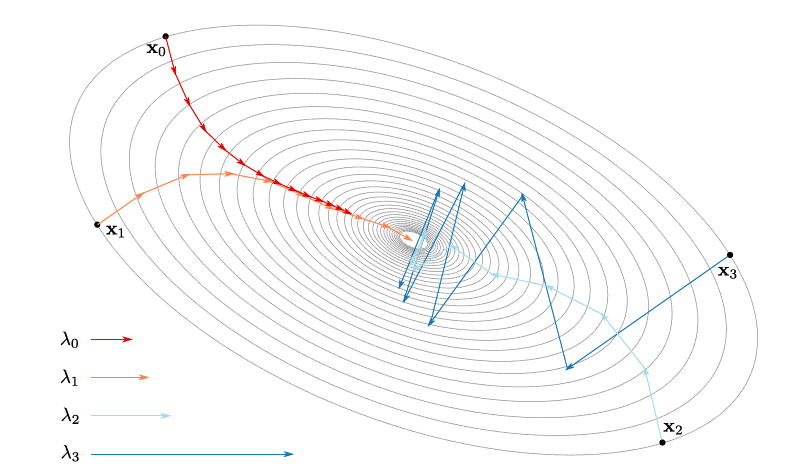
\includegraphics[width=\textwidth]{\imgpath/sgd_lr.png}
  \mycaption{Trajectories of SGD with different initial learning rates}{This
  figure illustrates the effect the step size has over the optimization process
  by showing the trajectory for $\eta = \lambda_i$ from equivalent starting
  points on a symmetric loss surface. Increasing the step size beyond
  $\lambda_3$ can cause the optimization procedure to diverge. Image
  taken from \cite{Ioannou2017thesis} Figure 2.7.}
  \label{fig:ch2:sgd_lr}
\end{figure}

\subsection{Momentum and Adam}
One simple and very popular modification to SGD is to add \emph{momentum}.
Momentum accumulates past gradients with an exponential-decay moving average and
continues to move in their direction. The name comes from the comparison of finding
minima to rolling a ball over a surface --
any new force (newly computed gradients) must overcome the current momentum of
the ball. This has a smoothing effect on noisy gradients.

We can achieve momentum by creating a \emph{velocity} variable $v_{t}$ and modify
\eqref{eq:ch2:gd} to be:
\begin{align}
  v_{t+1} &= \alpha v_t - \eta_k\dydx{J}{\theta} \label{eq:ch2:velocity}\\
  \theta_{t+1} &= \theta_t + v_{t+1}
\end{align}
where $0\leq\alpha<1$ is the momentum term indicating how quickly to `forget'
past gradients.

Another popular modification to SGD is the adaptive learning rate technique Adam
\cite{kingma_adam:_2014}. There are several other adaptive schemes such as
AdaGrad \cite{duchi_adaptive_2011} and AdaDelta \cite{zeiler_adadelta:_2012}, but
they are all quite similar, and Adam is often considered the most robust of the
three \cite{goodfellow_deep_2016}. The goal of all of these adaptive schemes is
to take larger update steps in directions of low variance, helping to minimize
the effect of large condition numbers we saw in \autoref{fig:ch2:gd_bounce}.
Adam does this by keeping track of the first $m_t$ and second $v_t$ moments of the
gradients:
\begin{align}
  g_{t+1} &= \dydx{J}{\theta} \\
  m_{t+1} &= \beta_1 m_{t} + (1-\beta_1)g_{t+1} \label{eq:ch2:adam_first}\\
  v_{t+1} &= \beta_2 v_{t} + (1-\beta_2)g_{t+1}^2
\end{align}
where $0 \leq \beta_1, \beta_2 < 1$. Note the similarity between updating the
mean estimate in \eqref{eq:ch2:adam_first} and the velocity term in
\eqref{eq:ch2:velocity}\footnote{The $m_{t+1}$ and $v_{t+1}$ terms are then
bias-corrected as they are biased towards zero at the beginning of training. We
do not include this for conciseness.}. The parameters are then updated with:
\begin{equation}
  \theta_{t+1} = \theta_t - \eta \frac{m_{t+1}}{\sqrt{v_{t+1}} + \epsilon}
\end{equation}
where $\epsilon$ is a small value to avoid dividing by zero.
